\documentclass[11pt,a4paper]{article}
\usepackage[utf8]{inputenc}
\usepackage[ngerman]{babel}
\usepackage{amsmath}
\usepackage{amsfonts}
\usepackage{amssymb}
\usepackage{scrpage2}\pagestyle{scrheadings}
\usepackage[pdftex]{graphicx}
\ihead{Thomas Verweyen (759743) \\ Norman Vetter (749229)}
\setheadsepline{0.2pt}
\begin{document}
\begin{center}
\section*{ Theoretische Informatik 1 \\ Übung Blatt 6}
\end{center}
\ \\ \ \\
\subsection*{Aufgabe 6.1}
\paragraph*{a)}\ \\
i)\\
\begin{tabular}{c|c}
enthalten & nicht enthalten\\
\hline
acab & bbb\\
cabb & abc \\
aacabbb & cba \\
aca & bacac \\
ca & cabc\\
\end{tabular}\ \\
ii)\\
\begin{tabular}{c|c}
enthalten & nicht entahlten\\
\hline
ba & abc\\
bc & cba \\
a & aabbcc\\
baab & abcabc\\
bab &  abbac\\
\end{tabular}\ \\
\paragraph*{b)}\ \\
i)\\
$G=(\{A,B,C,S\},\{0,1,2\},P,S)$:\\
$P:~S \rightarrow ABC, A \rightarrow \epsilon , A \rightarrow 2A , B \rightarrow \epsilon, B \rightarrow 0B, B \rightarrow 10B, C \rightarrow 1C, C \rightarrow 1$\\
ii)\\
Der Ausgangs RA konnte aufgrund der gegebenen Regeln auf RA'=$(0+12*)^*110(0+2)^*$ gekürzt werden.\\
$S \rightarrow ABC, A \rightarrow \epsilon, A \rightarrow 0A, A \rightarrow 1DA, D \rightarrow \epsilon, D  \rightarrow 2D, B \rightarrow 110,\\ C \rightarrow \epsilon, C \rightarrow 0C, c \rightarrow 2C$\\
\paragraph*{c)}\ \\
i) RA: $A=(b+c)^*$\\
\hspace*{12mm}$Ac^Ac^AaA+Ac^AaAc^A+AaAc^Ac^A$\\
ii) RA: $r^*sr^*s(r^*sr^*sr^*sr^*s)^*$\\
\subsection*{Aufgabe 6.2}
\paragraph*{a)}\ \\
i)\\
\begin{tabular}{ll}

$\Big ((R+S)(S+R)^* \Big )^*$&$\cong\Big ((R+S)(R+S)^* \Big )^*$\\
&$\cong \Big ((R+S))^+ \Big )^*$\\
&$\cong \Big ((S+R)^+ \Big )^++\epsilon$\\
&$\cong (S+R)^++\epsilon$\\
\end{tabular}
ii)\\
$S^*(R+S)^* \cong (S+RS)^*$  ist nicht Wahr, denn $R \subseteq S^*(R+S)^*,\\~aber~ R \nsubseteq (S+RS)^*$\\
ii)\\
Die Aussage: $(RTS + RT)^* RT \cong RT(SRT + RT)^*$ beschreibt eine alternierende Reihe bestehend aus RT's, wobei nach einem T und vor einem R ein S vorkommen kann aber nicht muss. Es ist dabei irrelevant ob das Teilwort vielleicht mit RTS beginnt und auf RT endet, oder ob es mit RT beginnt und auf SRT endet. Das resultierende Wort ist identisch. Die Möglichkeit RT's ein zu schieben verändert diesen Fakt nicht. Somit gilt diese Aussage für alle RA's R,S,T.\\
\ \\
\paragraph*{b)}\ \\
i)\\
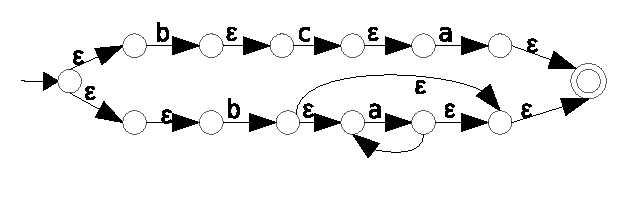
\includegraphics[scale=0.8]{6211.eps}\\
ii)\\
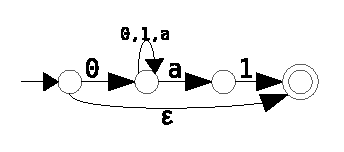
\includegraphics[scale=1]{6212.eps}\\
iii)\\
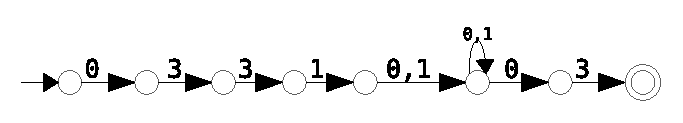
\includegraphics[scale=0.8]{6213.eps}\\
\subsection*{Aufgabe 6.3}
TO DO
\end{document}